\documentclass{article}
\usepackage[utf8]{inputenc}
\usepackage[margin = 0.8in]{geometry}
\usepackage{graphicx}
\usepackage{amsmath, amssymb}
\usepackage{subcaption}
\usepackage{multirow}
\usepackage{mathtools}
\usepackage{float}


\title{RBE549 - Homework 3}
\author{Keith Chester}
\date{Due date: September 22, 2022}

\begin{document}
\maketitle

\section*{Problem 1}

In this problem, we are tasked with using OpenCV to produce a sobel edge filter and a Marr-Hildreth detector. The code for this problem can be found in the associated $problem1.py$ code. The results are shown below.

\begin{figure}[H]
    \centering
    
\includegraphics[width = 0.45\textwidth]{imgs/original.jpg}
    \caption{We begin with our selfie image}
    \label{fig:original_image}
\end{figure}

\begin{figure}[H]
    \centering
    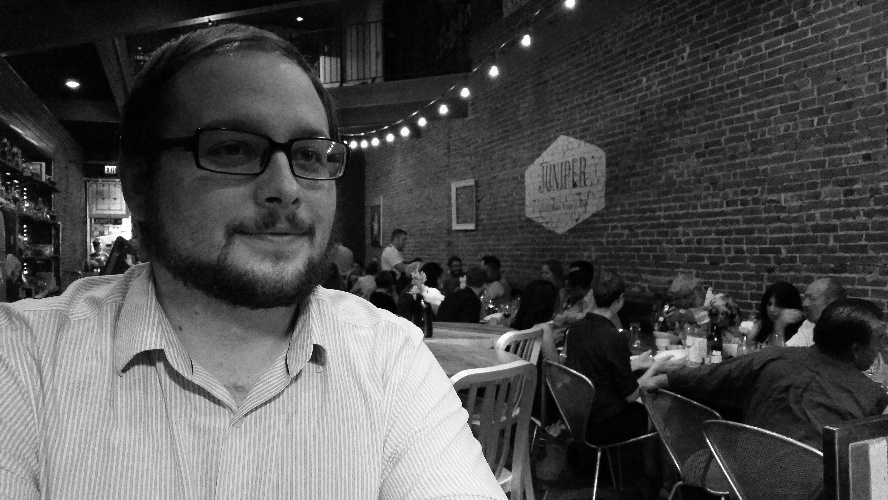
\includegraphics[width = 0.45\textwidth]{imgs/gray.jpg}
    \caption{We then convert it to greyscale to do our edge dection}
    \label{fig:grayscale}
\end{figure}

\begin{figure}[H]
    \centering
    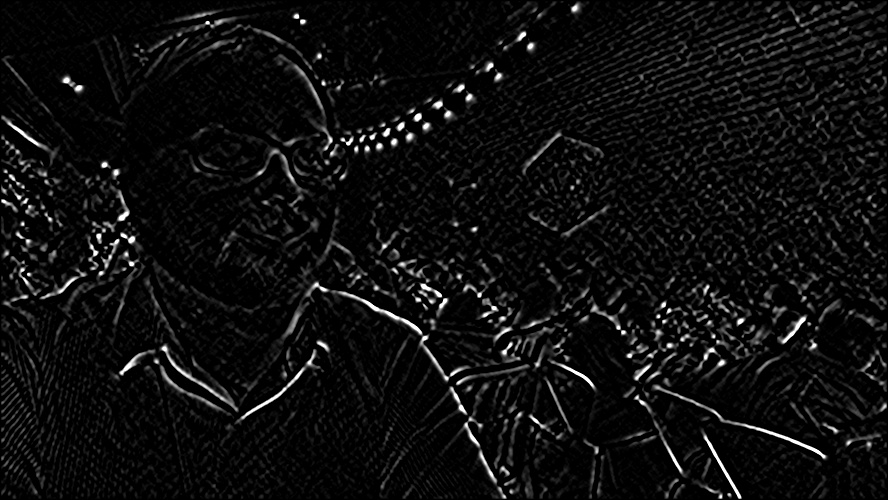
\includegraphics[width = 0.45\textwidth]{imgs/sobel.jpg}
    \caption{We gaussian blur and then apply a sobel filter}
    \label{fig:sobel}
\end{figure}

\noindent

After this, we then move through $\sigma=[1, 2, 4, 8, 16]$ to try a Marr-Hildreth filter. Here we perform the same operation - grayscale and Gaussian blur our images prior to passing it through the detector - but do additonal thresholding to try and improve results.

\begin{figure}[H]
    \centering
    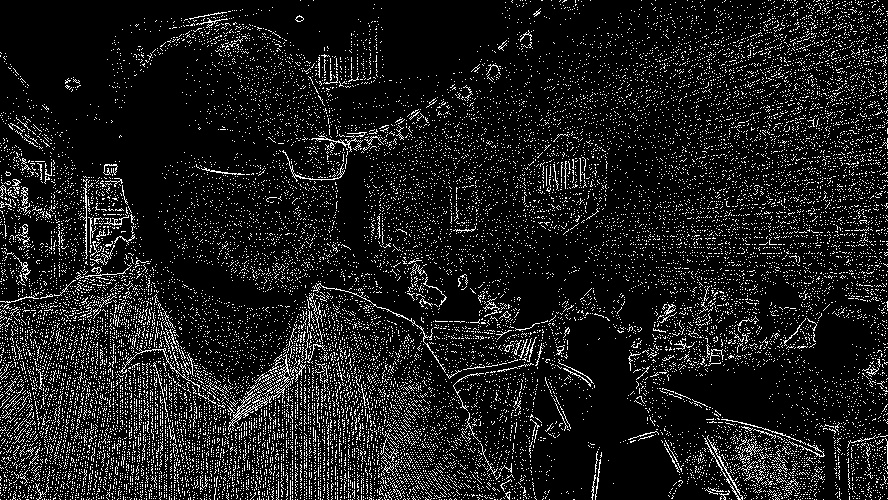
\includegraphics[width = 0.45\textwidth]{imgs/mh-1.jpg}
    \caption{$\sigma=1$}
    \label{fig:mh_1}
\end{figure}

\begin{figure}[H]
    \centering
    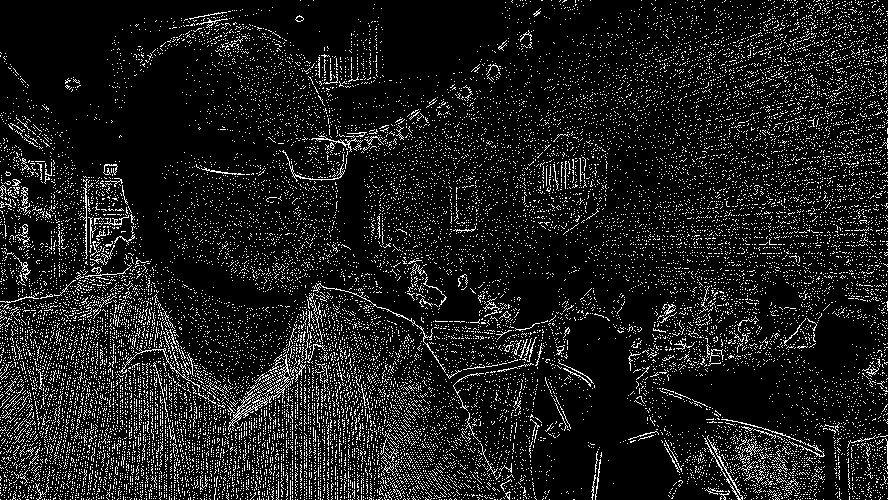
\includegraphics[width = 0.45\textwidth]{imgs/mh-2.jpg}
    \caption{$\sigma=2$}
    \label{fig:mh_2}
\end{figure}

\begin{figure}[H]
    \centering
    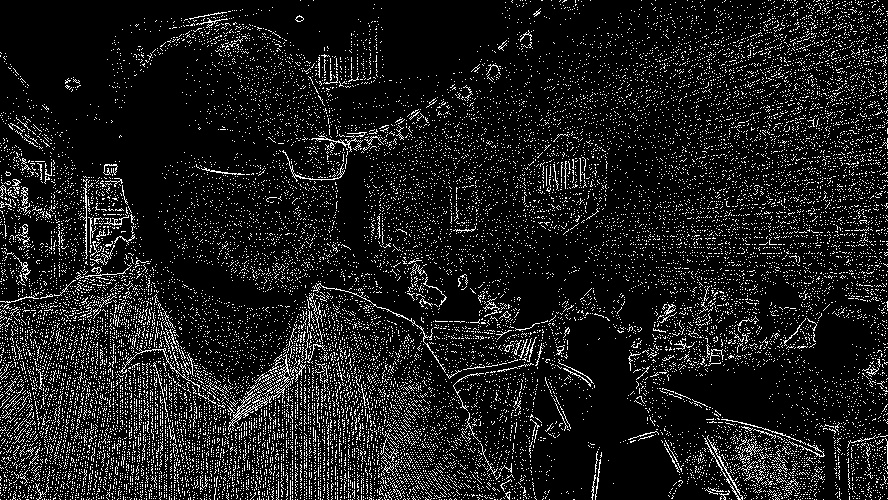
\includegraphics[width = 0.45\textwidth]{imgs/mh-4.jpg}
    \caption{$\sigma=4$}
    \label{fig:mh_4}
\end{figure}

\begin{figure}[H]
    \centering
    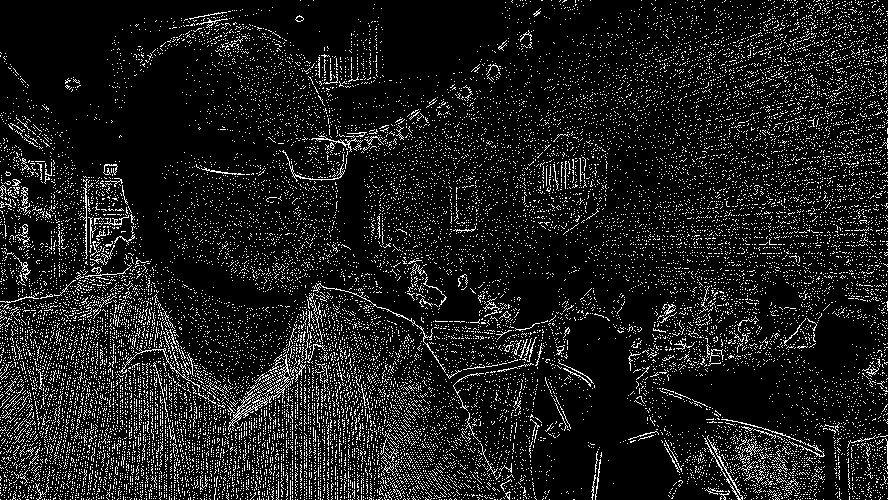
\includegraphics[width = 0.45\textwidth]{imgs/mh-8.jpg}
    \caption{$\sigma=8$}
    \label{fig:mh_8}
\end{figure}

\begin{figure}[H]
    \centering
    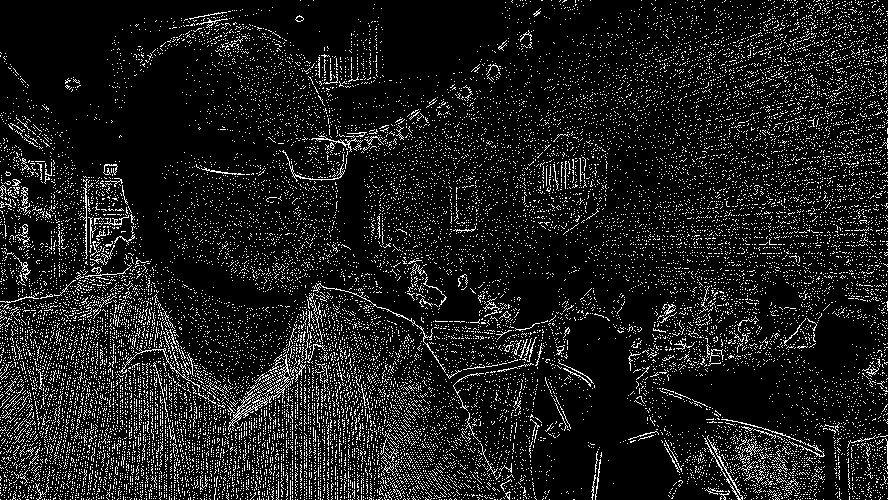
\includegraphics[width = 0.45\textwidth]{imgs/mh-16.jpg}
    \caption{$\sigma=16$}
    \label{fig:mh_16}
\end{figure}

As the $\sigma$ value raised, we begin to see better performance of the line detector. Unfortunately the original choice of the image is likely poor as the many defined lines of the brick wall behind the subject, paired with a straight vertical line shirt seems to introduce significant noise into the results.

\section*{Problem 2}

In this problem, we are tasked with proving that if $f(x)$ is an odd function and purely imaginiary (ie no real component), then the Fourier Transform of $f(x)$, $F(x)$ is both real and odd.

We start with defining $F(x)$:

\begin{equation}
    \int_{-\infty}^{\infty} f(x)e^{-j \omega x} dx
\end{equation}

\noindent ...and we can split this integral into two parts, specifically utilizing that $\int_{-A}^{A}$ can be split into muliple integrals of along the requested range, such that $\int_{-A}^0 + \int_0^A$ is equivalent.

\begin{equation}
    \int_{-\infty}^{0} f(x)e^{-j \omega x} dx + \int_{0}^{\infty} f(x)e^{-j \omega x} dx
\end{equation}

\noindent We can then exapnd this with an idenity:

\begin{equation}
    \int_{-\infty}^{0} f(x)(\cos(\omega x) - j\sin(\omega x)) dx + \int_{0}^{\infty} f(x)(\cos(\omega x) - j\sin(\omega x)) dx
\end{equation}

\noindent Similarly to before, we can utilize a property of integrals to further separate this - specifically that $\int (A(x)+B(X)) = \int A(x) + \int B(x)$.

\begin{equation}
    \int_{-\infty}^{0} f(x)\cos(\omega x) dx + \int_{-\infty}^{0} -j f(x) \sin(\omega x) dx + \int_{0}^{\infty} f(x)\cos(\omega x) dx + \int_{0}^{\infty} -j f(x) \sin(\omega x) dx
\end{equation}

\noindent We can reorder terms to isolate the cosine terms, and move $-j$ (since it's a constant) out of the integral:

\begin{equation}
    \int_{-\infty}^{0} f(x)\cos(\omega x) dx + \int_{0}^{\infty} f(x)\cos(\omega x) dx - j \int_{-\infty}^{0} f(x) \sin(\omega x) dx - j \int_{0}^{\infty} f(x) \sin(\omega x) dx
\end{equation}

\noindent To prove that a function is odd, we must show that $f(-x) = -f(x)$. However, we know that $\cos$ is an even function, meaning $f(-x)=f(x)$. thus if we were to plug in $-x$, our negative sign does not escape the cosine, resulting in a cancellation of terms. This ultimately leads us to:

\begin{equation}
    F(x) = -j \int_{-\infty}^{\infty} f(x) \sin(xt) dt
\end{equation}

\noindent Since $j$ is our imaginary component, and we have a singular component left, it shows that our Fourier transform is in fact completely imaginary. If we let $f(x) = jg(x)$ as $f(x)$ is purely imaginiary:

\begin{equation}
    F(x) = -j \int_{-\infty}^{\infty} jg(x) \sin(xt) dx = -j^2 \int_{-\infty}^{\infty} g(x) \sin(xt) = \int_{-\infty}^{\infty} g(x) \sin(xt)
\end{equation}

This result is an odd function (even or odd functions multiplied by an odd function is odd) with no imaginary components!


\section*{Problem 3}

In this problem we present an edge detector wherein we convolve an image $f(\vec{x})$ with:

\begin{equation}
     g_{\sigma_1} = \frac{1}{2\pi \sigma_1^2}e^{-\frac{|\vec{x}|^2}{2\sigma_1^2}}
\end{equation}

\noindent ...which forms $h_1(\vec{x})$. We then convolve $f(\vec{x})$ with $g_{\sigma_2}$ to get $h_2(\vec{x})$.

\noindent Then finally we compute $h_3(\vec{x}) = \frac{h_2(\vec{x}) - h_1(\vec{x})}{\sigma_2 - \sigma_1} $.

\subsection*{A}

First we aim to describe how $h_3(\vec{x})$ can be computed by a single convolution with some kernel $g(\vec{x})$. Since $h_1(\vec{x}) = f(\vec{x}) * g_{\sigma_1}(\vec{x})$, and $h_2(\vec{x}) = f(\vec{x}) * g_{\sigma_2}(\vec{x})$...  

\begin{equation}
  h_3(\vec{x}) = \frac{f(\vec{x})*g_{\sigma_2}-f(\vec{x})*g_{\sigma_1}}{\sigma_2 - \sigma_1}
\end{equation}

\noindent We can pull out the common $f(\vec{x})$ term and get:

\begin{equation}
    h_3(\vec{x}) = f(\vec{x})*\frac{g_{\sigma_2} - g_{\sigma_1}}{\sigma_2 - \sigma_1}
\end{equation}

\noindent ...which leads us to the convolution kernel of:

\begin{equation}
    g(\vec{x}) = \frac{g_{\sigma_2} - g_{\sigma_1}}{\sigma_2 - \sigma_1}
\end{equation}


\section*{Problem 4}
For this problem we look at two kernels that are used to detect diagonal edges:

\begin{equation}
    NE = \begin{bmatrix}
        1 & 1 & 0 \\
        1 & 0 & -1 \\
        0 & -1 & -1
    \end{bmatrix}
\end{equation}

\begin{equation}
    NW = \begin{bmatrix}
        0 & 1 & 1 \\
        -1 & 0 & 1 \\
        -1 & -1 & 0
    \end{bmatrix}
\end{equation}

\subsection*{A}

First, we are tasked with noting how these operators are located with the Sobel H and V operators. The Sobel H and V operators are horizontal and vertical line (respectively) detectors. They are shown below:

\begin{equation}
    V = \begin{bmatrix}
        -1 & 0 & 1 \\
        -2 & 0 & 2 \\
        -1 & 0 & 1 \\
    \end{bmatrix}
\end{equation}

\begin{equation}
    H = \begin{bmatrix}
        1 & 2 & 1 \\
        0 & 0 & 0 \\
        -1 & -2 & -1 \\
    \end{bmatrix}
\end{equation}

These operators are designed to detect either vertically oriented or horizontally oriented lines. Much like these operators, the presented $NW$ and $NE$ have a 0 designation across the target axis, but in our case looks for diagonal lines.

\subsection*{B}

Now we aim to suggest two ways to combine these operators into a singular kernel that can identify northeast or northwest diagonals together, and discuss the potential problems with these combinations.

First, the naive approach could be to just combine them with $0$ across the diagonal axes.

\begin{equation}
    \begin{bmatrix}
        0 & 1 & 0 \\
        1 & 0 & 1 \\
        0 & 1 & 0 \\
    \end{bmatrix}
\end{equation}

This has several issues. The first is that we don't actually detect or strength diagonal lines, as by looking for both we are essentially muting lines that are \textit{just} 45 degrees $NW$ $NE$. Also, our lack of negative values creating a significant value difference here between bottom and top part of the filter results in a poor filter with a lack of directionality, which can further diminish the ability to differentiate.

Another way to combine them would be to design a filter that would look heavily at diagonal lines and penalize anything else. Here I suggest the following filter:

\begin{equation}
    \begin{bmatrix}
        1 & -2 & 1 \\
        -2 & 4 & -2 \\
        1 & -2 & 1
    \end{bmatrix}
\end{equation}

...this filter would look for each without heavily penalizing directionality that could cause fainter diagonal lines to be lost.

\subsection*{C}

This problem asks us to express $NW$ as a convolution of an unknown $2x2$ operator with the kernel of:

\begin{equation}
    \begin{bmatrix}
        0 & 1 \\
        -1 & 0 \\
    \end{bmatrix}
\end{equation}

\noindent ...or, if we labeled the above as $h(x)$, find $g(x)$ such that $g(x)*h(x) = NW$. The resulting matrix for $g(x)$ is:

\begin{equation}
    \begin{bmatrix}
        1 & 1 \\
        1 & 1 \\
    \end{bmatrix}
\end{equation}

\section*{Problem 5}

We look at the outcome of convolving a Sobel vertical edge detector ($V$) with a $3x3$ blurring mask ($B$)

\begin{equation}
    V = \begin{bmatrix}
        -1 & 0 & 1 \\
        -2 & 0 & 2 \\
        -1 & 0 & 1 \\
    \end{bmatrix}
\end{equation}

\begin{equation}
    B = \begin{bmatrix}
        2 & 3 & 2 \\
        3 & 4 & 3 \\
        2 & 3 & 2 \\
    \end{bmatrix}
\end{equation}

\subsection*{A}

We ask - what is the result of the combined convolutional mask for applying $V$ first, and then $B$? If we perform the convolution, we get a matrix that is a $5x5$:

\begin{equation}
    \begin{bmatrix}
        -2 & -3 & 0 & 3 & 2 \\
        -7 & -10 & 0 & 10 & 7 \\
        -10 & -14 & 0 & 14 & 10 \\
        -7 & -10 & 0 & 10 & 7 \\
        -2 & -3 & 0 & 3 & 2 \\
    \end{bmatrix}
\end{equation}

\subsection*{B}

We are asked if convolving with $B$ first, then $V$ produces different results than convolving with $V$ first, and then $B$. The answer is \emph{no} - convolution has a commutative property - $f(x)*g(x) = g(x)*f(x)$. Thus we would have the same result we found in part A of this question.

\subsection*{C}

In this part, we're asked if the convolution mask of $V*B$ seperable into a convolution of x-only and y-only masks. The answer here is \emph{no} as well. In order for a convoluton mask to be seperable, the resulting matrix must have a rank of $1$. The rank of our resulting mask is $2$, thus precluding us from finding a seperable convolution.


\end{document}